\section{Energy minimization}
		As it can be expected, the values of the energy can depend heavily with respect to the variational parameters, so the optimal value must be found. This usually means finding the minimum value, and the first option would obviously be just a brute force search, but this is not efficient and there are better alternatives. Among these, we can find the steepest descent method, the conjugate gradient method and the Newton-Raphson method (also known as simply Newton's method\footnote{It should be remarked that what we today commonly refer to as ``Newton's method'' in fact is Raphson's simplification of the method. However, Newton isn't mentioned in Raphson's presentation of the method; Raphson evidently considered  his method to be fairly different than Newton's. That Raphson worked independently of Newton is however doubtful. But the ``Newton-Raphson method'' is therefore a more fitting denomination for the method than ``Newton's method'' \cite{cajori1911}.}) \cite{newton1671} \cite{raphson1702}. The first two offer the possibility of finding a minimum in a multivariate space, while the Newton-Raphson method only allows searching in one dimension, but is simpler and faster.

		Since these methods don't find minima but the zeros of a function, the derivative of said function is needed. But there is no analytical expression for the local energy, so a workaround must be used. It is possible to find an analytical expression of this derivative as a function of the values of the local energy and the logarithmic derivative of the wave function. Following \cite{mortens_notes} the expression for the derivative with respect to parameter $c$ is 
		%\todo{remove/redo reference}

		\begin{equation}
		\frac{\partial E}{\partial c}=2\left[\langle E_L\frac{\partial\ln{\Psi}}{\partial c}\rangle-E\langle\frac{\partial\ln{\Psi}}{\partial c}\rangle\right],
		\end{equation}

		or more explicitly

		\begin{equation}
		\frac{\partial E}{\partial c}=\frac{2}{N}\left[\sum_{i=1}^N\left(\left[E_L\left(c\right)\right]_i\left[\frac{\partial\ln{\Psi}}{\partial c}\right]_i\right)-\frac{1}{N}\sum_{i=1}^N\left(\left[E_L\left(c\right)\right]_i\sum_{j=1}^N\left[\frac{\partial\ln{\Psi}}{\partial c}\right]_j\right)\right],
		\end{equation}

		where the indices's $i$ and $j$ run through all the time steps independently of each other. In our case, we are going to derive with respect to $\beta$ only, because we are only interested in minimization in that direction. Since the derivative is composed of three parts, two for the Slater determinants and one for the Padé-Jastrow interaction part, we get

		\begin{eqnarray*}
		\frac{\partial\ln{\Psi}}{\partial\beta} & = & \frac{\partial\ln{\Psi_{SD\uparrow}}}{\partial\beta}+\frac{\partial\ln{\Psi_{SD\downarrow}}}{\partial\beta}+\frac{\partial\ln{\Psi_J}}{\partial\beta}=\frac{\partial\ln{\Psi_J}}{\partial\beta}\\ 
		& = & \frac{\partial\left(\sum_{i<j}\frac{ar_{ij}}{1+\beta r_{ij}}\right)}{\partial\beta} = \sum_{i<j}\frac{-ar_{ij}^2}{\left(1+\beta r_{ij}\right)^2}.
		\end{eqnarray*}

		So the resulting expression is

		\begin{equation}
		\begin{split}
		\frac{\partial E}{\partial\beta}= & \frac{2}{N}\left[\sum_{i=1}^N\left(\left[E_L\left(\beta\right)\right]_i\left[\sum_{k<l}\frac{-ar_{kl}^2}{\left(1+\beta r_{kl}\right)^2}\right]_i\right) \right.\\ 
		& \left. - \frac{1}{N}\sum_{i=1}^N\left(\left[E_L\left(\beta\right)\right]_i\sum_{j=1}^N\left[\sum_{k<l}\frac{-ar_{kl}^2}{\left(1+\beta r_{kl}\right)^2}\right]_j\right)\right],
		\end{split}
		\end{equation}

		with $k$ and $l$ running through the electrons. We assume that we need to minimize with respect to one variable, $\beta$, and choose the Newton-Raphson method for its simplicity. This method additionally requires the derivative of the function ($\partial E/\partial\beta$ in this case), but it's not possible to simply derive with respect to $\beta$ again because there is no analytical expression for $E_L\left(\beta\right)$. Therefore we must resort to numerical derivation. A simple, first oder finite difference method can be used for this

		\begin{equation}
		\frac{\partial^2 E}{\partial\beta^2}=\lim_{h\to 0}\frac{\frac{\partial^2 E\left(\beta+h\right)}{\partial\beta^2}-\frac{\partial^2 E\left(\beta\right)}{\partial\beta^2}}{h}.
		\end{equation}

		With this the Newton-Raphson method can be implemented in a straight forward manner with one simple equation

		\begin{equation}
		\beta_{i+1}=\beta_i-\frac{\frac{\partial E}{\partial\beta}}{\frac{\partial^2 E}{\partial\beta^2}},
		\end{equation}

		where the index $i$ represents the iterations of the Newton-Raphson method, not the iterations of the Monte Carlo loop; for each iteration of this index a whole Monte Carlo loop is performed. In the first iteration a seed must be provided for the random generator. Depending on the guess for this seed, the method's performance will be better or worse.

		There is one catch, the values of the first derivative are computed as a part of the Monte Carlo loop, and are thus susceptible to a certain degree of randomness. This variability introduces some uncertainty in each iteration. Basically, we are not applying the method to a function, but to a scattered point cloud from which we sample points one at a time. This, coupled with the fact that the second derivative is obtained numerically from two points of that cloud, made the method show poor results, namely slow convergence to values that apparently depended heavily on the seed choice. To circumvent this issue, a different, yet similar method was used, the bisection method

		The bisection method is similar to the Newton-Raphson method, but it only needs the function that has the roots we want to find. And, instead of a point seed, it needs an interval seed. The method exploits Bolzano's theorem in said interval: if the values of the function (the derivative of the local energy in this case) in the extremes have different signs, the existence of at least one root is guaranteed. By evaluating the function in the midpoint of the interval, it is possible to know in which half of it the root lies, and thus the interval can be reduced to one of its halves. This process is repeated until a certain tolerance is reached and the root is obtained. In our case we don't have to worry about multiple roots because we know that there is only one minimum, the only problem is choosing the appropriate intervals so that the method can find the root.

		%\begin{figure}
		%	\centering 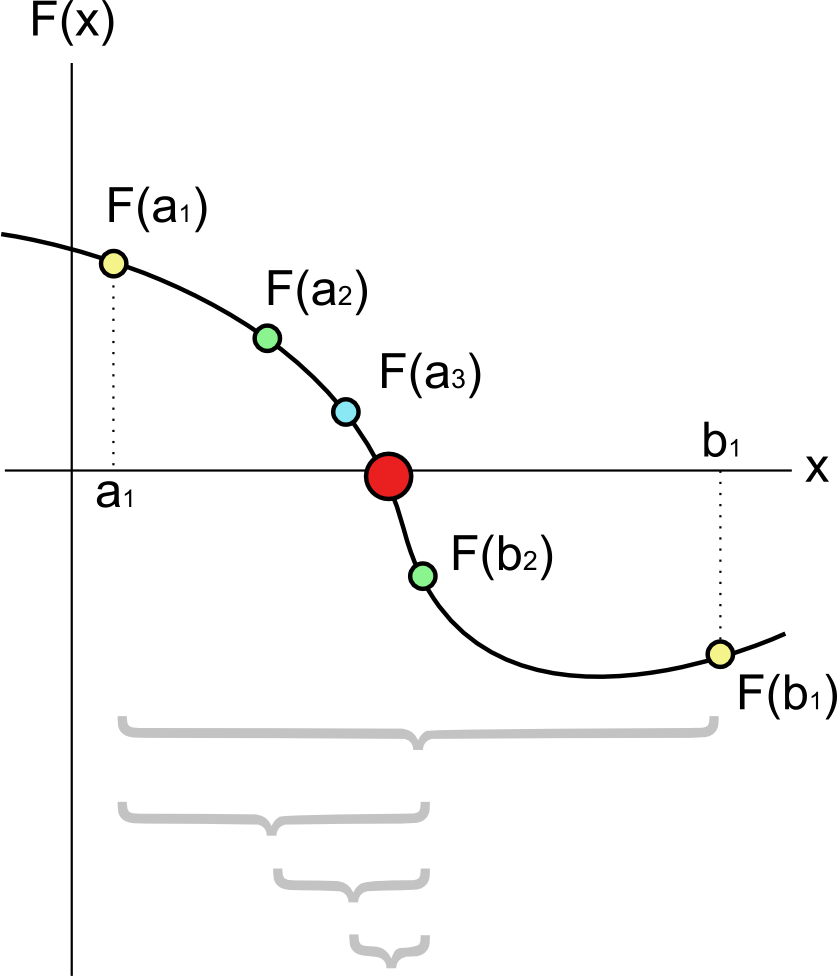
\includegraphics[width=0.45\linewidth]{content/Theory/figures/Bisection_method}
		%	\protect\caption{Schematic representation of the bisection method: in each iteration the interval is halved in two and it converges linearly to the solution}
		%\end{figure}

		The main advantage here compared to the Newton-Raphson method is that the sensibility to the values of the function is much smaller because only the sign of the function values is important (and this only becomes a problem when we are already very close to the root). The other advantage is the robustness and simplicity, the method will converge no matter what if the appropriate interval is chosen, which is not something very complicated to guess and can be checked quite fast in case it's not so obvious. The downside is the linear, comparatively slow convergence. But in this case, due to the the imprecision in obtaining the values of the derivative of the local energy, the Newton-Raphson method becomes relatively slow as well, so it is not actually a problem for our purposes.

		
